%!TEX root = ../talk.tex

\section{Introduction}\label{sec:intro}

%%%
\subsection{Background}
%%%

\begin{frame}
  \MyLogo
  \frametitle{Machine Learning}  

\begin{itemize}

\item ML gives computers the ability to learn without being explicitly programmed {\footnotesize\color{DarkOrchid}[Samuel 1959]}

\item ML explores the study and construction of algorithms that can learn from and make predictions on data

\item Data mining, computational statistics, optimization, ...

\item Fourth paradigm, big data, deep learning, artificial intelligence 

\end{itemize}

\end{frame}

%%%

\begin{frame}
  \MyLogo
  \frametitle{General Tasks of ML}

\begin{itemize}

\item Classification: Inputs are divided into two or more classes, and the learner must produce a model that assigns unseen inputs to one or more (multi-label classification) of these classes

\item Clustering: Inputs are divided into groups. Unlike in classification, the groups are not known beforehand, making this typically an unsupervised task

\item Regression: Similar to classification, but the outputs are continuous rather than discrete

\item Other tasks: density estimation, dimensionality reduction, ...

\end{itemize}

\end{frame}

%%%
\subsection{General ML code}
%%%

\begin{frame}
  \MyLogo
  \frametitle{Packages for General Machine Learning}  
\small

\structure{What is the purpose?}
\begin{itemize}
\item Solving problems from practical applications (user interface)
\item Developing algorithms and optimizing implementation (development)
\item Theoretical analysis for machine learning
\end{itemize}

\structure{What do we want for a ML package?}
\begin{itemize}
\item Easy for new tasks and new network structures (less steep learning curve)
\item Easy for debugging (with good support and large community)
\item Performance and scalability
\end{itemize}

\vskip -5pt
\begin{figure}[htbp] %  figure placement: here, top, bottom, or page
   \centering
   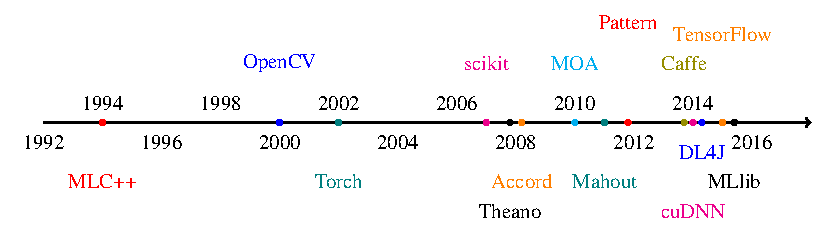
\includegraphics[width=\linewidth]{figures/ML.pdf} 
\end{figure}

\end{frame}

%%%
\subsection{DL code}
%%%

\begin{frame}
  \MyLogo
  \frametitle{Deep Learning}  

\end{frame}
